%\subsection[$\vec{p}$ and $\Delta \vec{p}$ In Two and Three Dimensions, Part II]{Momentum and Change in Momentum In Two and Three Dimensions, Part II}
\subsection{Heavy Ball Swung in a Horizontal Circle -- String Breaks}
\label{act7.2.2}

%Discuss and put on the board the following follow-up questions to each FNT. You will have 8-10~minutes per FNT. Each FNT will be followed by a WC discussion with student presentations.
\label{act7.2.2-1}
\begin{fnt}
	\label{fnt7.2.1-2}

Turn to the \pModel{} summary page and do the following:

\begin{enumerate}
	\item Use the model relationships found there to analyze each physical situation, and
	\item Make logical arguments that would convince another physics student of your response to the following prompts.
\end{enumerate}

\noindent Remember that a momentum conservation law requires you to compare a quantity at two times so you must always consider an initial time and a final time.\\

\noindent\parbox[t]{\textwidth}{%
      \vspace{-3mm}
      \begin{wrapfigure}[10]{r}{3cm}
        \centering
        \vspace{-\baselineskip}%\vspace{-10pt}
			\begin{tikzpicture}[decoration={markings,mark=at position 0.5*\pgfdecoratedpathlength with {\arrow[thick]{>}},mark=at position 1*\pgfdecoratedpathlength with {\arrow[thick]{>}}},thick,scale=0.8, every node/.style={transform shape},background rectangle/.style={fill=white}, show background rectangle]{r}{2cm}
  	\centering
		\node[inner sep=0pt] (fingers) at (-.32,.16) {
\includegraphics[width=1cm]{pinchedFingers.png}};
		\draw[postaction={decorate},dashed] (0,0) circle [radius=1.5cm];
		\draw (0,0) -- (1.06,-1.06);
		\draw[fill=gray] (1.06,-1.06) circle (.1) node[right=2pt] {$P$};
	\end{tikzpicture}
\end{wrapfigure}
\noindent A heavy ball is attached to a string and swung in a circular path counter-clockwise in a horizontal plane as illustrated in the diagram to the right.  At point $P$ indicated in the diagram, the string suddenly breaks and the ball is released.  If these events were observed from directly above, draw the path the ball takes immediately after the string breaks.
}
\end{fnt}
\begin{enumerate}
	\item On the board, draw a physical picture of the situation. Make sure to include from 10\textdegree{} before the string breaks until after the string breaks.
	\item On the board, make a \pchart{} for this phenomenon, taking the initial point to be about 10\textdegree{} before the string breaks and the final point to be immediately before the string breaks.
	\item On the board, make a second \pchart{} for this phenomenon, taking the initial point to be immediately after the string breaks and the final point to be after the ball has gone a short distance.
	\item Use your charts to explain the path of the heavy ball, before and after the string breaks.
\end{enumerate}
\WCD

\newpage
\subsection{An Asteroid Moving in a Straight Line Receives a Push at Right Angles}
\label{act7.2.2-2}

The diagram below depicts an asteroid, moving with a \textbf{constant velocity}, from point $a$ to point $b$ in space where there is no air resistance. When the asteroid reaches point $b$, an alien (who decides the asteroid is in her way) applies a force for an instant in the direction of the solid arrow. 

\begin{center}
	\begin{tikzpicture}
		\node[inner sep=0pt] (asteroid) at (0,0) {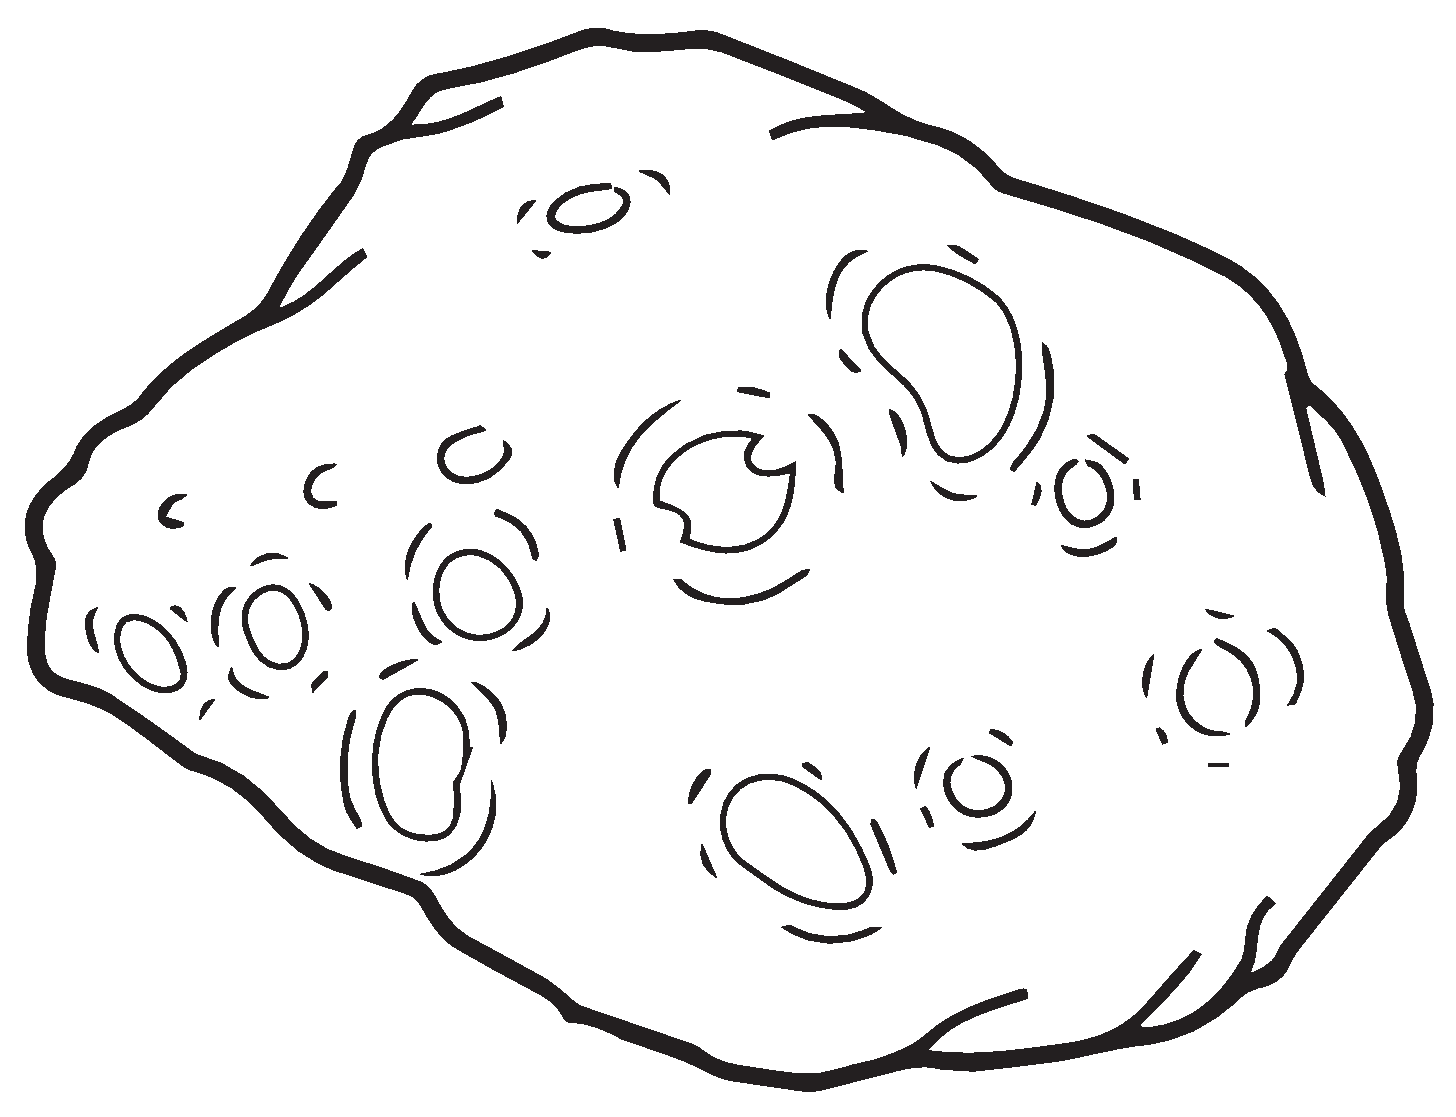
\includegraphics[width=3cm]{asteroid.eps}} node[right=1.5cm] {--- $b$};
		\draw[dashed,thick,-Stealth] (0,-4) -- (0,-1.1);
		\draw (2,-4) node {--- $a$};
		\node[inner sep=0pt] (alien) at (-3.7,0) {
\includegraphics[width=1.8cm]{alien.eps}};
		\draw[thick,-Stealth] (-3,0) -- (-1.5,0);
	\end{tikzpicture}
\end{center}

\begin{fnt}
	\label{fnt7.2.1-3}

Draw the path of the asteroid \textbf{after} the alien applies the force.
\end{fnt}

\begin{enumerate}
	\item On the board, make a \pchart{} for this phenomenon taking the initial point to be just before the push and the final point to be just after the push.
		\label{act7.2.2-2a}
	\item On the board, make a second \pchart{} for this phenomenon taking the initial point to be the same point as the final point in \eqref{act7.2.2-2a} and the final point to be after the asteroid has traveled some distance.
		\label{act7.2.2-2b}
	\item Use your \pcharts{} to explain the path of the asteroid.
	\item Considering your work above in \eqref{act7.2.2-2a} what is the predominant effect of the push?
\end{enumerate}
\vspace{-6pt}
\WCD
\vspace{6pt}
%\subsection{Asteroid moving in a straight line receives a push at right angles}
%\label{act7.2.2-3}

\begin{fnt}
	\label{fnt7.2.1-4}

Along the path you chose in \ref{fnt7.2.1-3}, how does the speed of the asteroid vary \textbf{after} receiving the ``kick''?  Is the velocity changing in direction? Is it increasing, decreasing or remaining the same in magnitude? Describe the motion.
\end{fnt}

\begin{enumerate}\setcounter{enumi}{4}
	\item On the board, use the appropriate \pchart{} from %\hyperref[act7.2.2-2]{\ref*{act7.2.2-2}}
	\eqref{act7.2.2-2a} and \eqref{act7.2.2-2b}
	 to justify your answer to this FNT.
\end{enumerate}
\vspace{-6pt}
\WCD
\vspace{6pt}
%\subsection{Asteroid moving in a straight line receives a push at right angles}
%\label{act7.2.2-4}

\begin{fnt}
	\label{fnt7.2.1-5}

Identify the forces acting on the asteroid, \textbf{after} the alien is finished applying the force.
\end{fnt}

\begin{enumerate}\setcounter{enumi}{5}
	\item On the board, use the appropriate \pchart{} from %\hyperref[act7.2.2-2]{\ref*{act7.2.2-2}}
	\eqref{act7.2.2-2a} and \eqref{act7.2.2-2b}
	 to make a scaled force diagram to answer this FNT.
\end{enumerate}
\vspace{-6pt}
\WCD

\subsection{A Ball Is Dropped and Bounces}
\label{act7.2.2-5}

\begin{fnt}
	\label{fnt7.2.1-6}

When a rubber ball dropped from rest bounces off the floor, its direction of motion is reversed because
\begin{enumerate}[(a)]
	\item energy of the ball is conserved;
	\item momentum of the ball is conserved;
	\item the floor exerts a force on the ball that stops its fall and then drives it upward;
	\item the floor is in the way and the ball has to keep moving;
	\item none of the above.
\end{enumerate}
\end{fnt}

\noindent On the board, make a \pchart{} (include a force diagram) that helps make sense of this situation and helps you to answer the question in this FNT.

\vspace{6pt}
\WCD









 
